\subsection{Experimental validation}
In order to further validate the model, the laboratory experiments from Ogorodnikova \textit{et al} \cite{ogorodnikova_deuterium_2003} are simulated.
We choose these particular experiments as it has already been simulated several times in \sidecite{ogorodnikova_deuterium_2003,hodille_macroscopic_2015,bonnin_rate_2015,benannoune_numerical_2019}.
Therefore, this simulation can be used as a benchmark case for FESTIM.\\
In this experiment, after deuterium (D) implantation in hot-rolled tungsten (W), Temperature Programmed Desorption (TPD) is performed.
TPD consists in heating the sample with a well controlled temperature ramp and measure with a mass spectrometer the evolution of the amount of desorbed particles with respect to temperature.
This results in a TPD spectrum.
In order to reproduce this spectrum, three phases are simulated.

The first one is the implantation phase where the source term in Equation \ref{eq:mobile} is $S_{ext} = (1-r) \cdot \varphi \cdot f(x)$, $r$ being the reflection coefficient (\textit{i.e.} the proportion of particles which are reflected from the surface to the plasma), $\varphi$ the incident ion flux in $\si{m^{-2}.s^{-1}}$ and $f(x)$ a Gaussian distribution with $R_p$ its mean value and $\sigma$ its width.
The parameters of $f(x)$ are determined with the software SRIM \sidecite{ziegler_srim_2010}.
This phase lasts $t_\mathrm{imp}$ and the temperature is $T = T_\mathrm{imp}$.\\
The second phase is the resting period where the source is turned off (\textit{i.e.} $S_{ext} = 0$) for a time $t_\mathrm{rest}$ at $T = T_\mathrm{rest}$.\\
Finally, the last period is the TPD where temperature is increased linearly with a given heating ramp $\beta$.\\
In order to fit the experimental results, three traps are needed: two intrinsic traps and one extrinsic trap to account for the creation of ion-induced defects during the implantation.
Extrinsic traps can be created by either supersaturation of HIs in the implantation range $f(x)$ creating monovacancies \sidecite{sun_critical_2014, fernandez_hydrogen_2015, ohsawa_thermodynamics_2015, kato_super-saturated_2015,hodille_hydrogen_2018}, that can lead to vacancy clusters and bubbles \sidecite{ogorodnikova_deuterium_2003, condon_hydrogen_1993} or local stress field \sidecite{poon_flux_2002, alimov_depth_2005}.
According to \sidecite{hodille_hydrogen_2018}, mono-vacancies can be created in the implantation zone when W is exposed to D ion flux if the flux is higher than a threshold limit for a given temperature.
At the temperature of the considered experiment (300 K), the threshold flux is ~$10^{18}$ $\: \si{m^{-2}s^{-1}}$ which is lower than the flux in the experiment (see Table \ref{tab:parameters validation}).


The evolution of the extrinsic trap density is given by Equation \ref{eq:extrinsic trap}.
 
\begin{equation}
    \begin{split}
        \frac{dn_3}{dt}  = (1-r)\: \varphi\:  \bigg[ & \left(1-\frac{n_3}{n_{3a_\mathrm{max}}}\right) \:\eta_a  \:f(x) \\  + &\left(1-\frac{n_3}{n_{3b_\mathrm{max}}}\right) \:\eta_b  \:\theta_{xp}(x) \bigg]
    \end{split}
    \label{eq:extrinsic trap}
\end{equation}
 
where $\theta_{xp}(x) = \frac{1}{x_p}\quad \forall x < x_p$, $\eta_a$ and $\eta_b$ are the rates of traps creation and ${n_{3a_\mathrm{max}}}$ and ${n_{3b_\mathrm{max}}}$ are their maximum values.
This formulation follows the one proposed in \sidecite{hodille_macroscopic_2015,bonnin_rate_2015} based on the expression of Ogorodnikova \textit{et al.} \sidecite{ogorodnikova_deuterium_2003}.

All the above parameters are presented in Table \ref{tab:parameters validation}. These parameters are in good agreement with those used in \sidecite{hodille_macroscopic_2015,bonnin_rate_2015,benannoune_numerical_2019}.
\begin{table} [ht]
    \centering
    \begin{tabular}{p{2.3cm} p{2cm} r}
        %\hline
        Parameter & Units & Value \\
        \hline
        \\
        $\rho_W$ & $\si{m^{-3}}$ &$6.3 \times 10^{28}$ \\
        $n_\mathrm{solute}$ & & $6 \:\rho_W$\\
        $n_1$ & & $1 \times 10 ^{-3} \rho_W$ \\
        $n_2$ &  & $4 \times 10 ^{-4} \rho_W$ \\
        $n_{3a_\mathrm{max}}$ & & $1 \times 10 ^{-1} \rho_W$ \\
        $n_{3b_\mathrm{max}}$ & & $1 \times 10 ^{-2} \rho_W$ \\
        \\
        $E_\mathrm{diff}$ & $\si{eV}$ & $0.39$ \\
        $E_1$ &  & $0.87$ \\
        $E_2$ &  & $1.00$ \\
        $E_3$ &  & $1.50$ \\
        \\
        $\eta_a$ & - & $6 \times 10 ^{-4}$ \\
        $\eta_b$ & - & $2 \times 10 ^{-4}$ \\
        \\
        $\lambda$ & $\si{m}$ & $110 \times 10 ^{-12}$  \\
        $x_p$ & & $1 \times 10 ^{-6}$ \\
        $R_p$ & & $4.5 \times 10^{-9}$ \\
        $\sigma$ & & $4.5 \times 10^{-9}$ \\
        \\
        $T_\mathrm{imp}$ & $\si{K}$ & 300 \\
        $T_\mathrm{rest}$ & & 300 \\
        \\
        $t_\mathrm{imp}$ & $\si{s}$ & 400 \\
        $t_\mathrm{rest}$ & & 50 \\
        \\
        $\nu_0$ & $\si{s^{-1}}$ & $10 ^{13}$ \\
        $\beta$ & $\si{K.s^{-1}}$ & 8 \\
        $D_0$ & $\si{m^2.s^{-1}}$ & $4.1 \times 10 ^{-7}$ \\
        $\varphi$ & $\si{m^{-2}.s^{-1}}$ & $2.5 \times 10 ^{19}$ \\
        $r$ & - & 0 \\
        \\
    \end{tabular}
    \caption{Parameters used for experimental validation}
    \label{tab:parameters validation}
\end{table}

The simulated TPD spectrum is represented on Figure \ref{fig:TPD spectrum}.
\begin{figure} [ht]
    \centering

    \begin{overpic}[width=1\linewidth]{"Figures/Chapter3/Comparaison exp-FESTIM"}
    \put(35,55){$\Bigg\uparrow$}
    \put(44.5,45){$\Bigg\uparrow$}
    \put(63.5,20){$\Bigg\uparrow$}
    \end{overpic}
    \caption{TPD spectrum simulated by FESTIM compared to experimental data of Ogorodnikova \textit{et al.} \cite{ogorodnikova_deuterium_2003}.}
    \label{fig:TPD spectrum}
\end{figure}

One can see that the spectra produced by FESTIM and by Ogorodnikova \textit{et al.} \sidecite{ogorodnikova_deuterium_2003} are in good agreement.
One peak can be distinguished at 450 K with two pronounced shoulders at 500 K and 620 K.
As denoted by the arrow in Figure \ref{fig:TPD spectrum}, the peak at 450 K corresponds to the detrapping from the low-energy high-concentration trap and the shoulders at 500 K and 620 K correspond to detrapping from 1.00 eV and 1.50 eV trap, respectively.
\subsection{Analytical verification}
\subsubsection{Analytical verification against a known solution} \label{analytical}

Although validation against experiments could show that FESTIM is able reproduce the data with a given set of parameters, objective verification against analytical solutions is first required to ensure that the governing Equations \ref{eq:mobile} and \ref{eq:trapped} are solved correctly.

For this verification case, a 1D slab is considered with a thickness $l$.
The concentration of mobile particles was set to $c_0$ on one side of the slab and set to zero on the other side.
Only one trap is considered in this case and its density $n_1$ is homogeneously distributed.

The trapping parameter $\zeta$ is defined in \sidecite{longhurst_verification_2005} as follow:
\begin{equation}
    \zeta = \frac{\lambda^2 \: n_\mathrm{solute} \: \nu_0}{D_0 \: n_1}\exp\bigg(\frac{E_\mathrm{diff} - E_1}{k_B \: T}\bigg) + \frac{c_m}{n_1}
\end{equation}

In our case, we choose the detrapping energy $E_1$, the concentration $c_0$ and the temperature $T$ so that $\zeta \gg \frac{c_m}{n_1}$.
This is known as the \textit{effective diffusivity regime} where the diffusion is almost identical to the case where there are no traps.
The coefficient $D$ is then replaced by an effective diffusion coefficient:
\begin{equation}
    D_\mathrm{eff} = \frac{D}{1+\frac{1}{\zeta}}
\end{equation}
The particle flux at the background surface is expressed in $\SI{}{H.m^{-2}.s^{-1}}$ and finally defined in \sidecite{longhurst_verification_2005} by:
\begin{equation}
    \varphi_H(t) = \frac{c_0 D}{l}\bigg[1+2\sum_{m=1}^{\infty}(-1)^m \exp\bigg(-m^2\frac{\pi^2 \:D_\mathrm{eff} \: t}{l^2}\bigg)\bigg]
\label{eq:flux analytical}
\end{equation}
All the parameters are defined in Table \ref{tab:parameters analytical verification}.
These parameters have been chosen for the sake of verification and do not necessarily represent realistic conditions as verification is a mathematical exercise.
\begin{table}
    \centering
    \begin{tabular}{p{2.3cm} p{2cm} r}
        Parameter & Units & Value \\
        \hline
        \\
        $\rho$ & $\si{m^{-3}}$ &$\SI{3.16e22}{}$ \\
        $n_1$ & & $\SI{1.00e-1}{} \rho$ \\
        $c_0$ & & $\SI{1.00e-4}{} \rho$\\
        $n_\mathrm{solute}$ & & $2 \:\rho$\\
        \\
        $E_1$ & $\si{eV}$ & $\SI{8.6e-3}{}$ \\
        $E_\mathrm{diff}$ & & $0$ \\
        \\
        $\lambda$ & $\si{m}$ & $\SI{3.16e-8}{}$  \\
        $l$ & & $\SI{5e-5}{}$\\
        \\
        $T$ & $\si{K}$ & 1000 \\
        \\
        $t_f$ & $\si{s}$ & \SI{e-8}{} \\
        $\nu_0$ & $\si{s^{-1}}$ & $\SI{e13}{}$ \\
        $D_0$ & $\si{m^2.s^{-1}}$ & $1$ \\
        \\
    \end{tabular}
    \caption{Parameters used for the analytical verification}
    \label{tab:parameters analytical verification}
\end{table}
One can notice on Figure \ref{fig:FESTIM vs analytical} that the numerical results are in good agreement with the analytical solution.
The maximum error between analytical and numerical solutions is calculated to be \SI{6.56e20}{H.m^{-2}.s^{-1}} with 50000 piecewise linear elements (P1) which corresponds to \SI{1}{\%} of the maximum value.
According to finite elements theory, this value will decrease with the stepsize and with the element size.
\begin{figure}
    \centering
    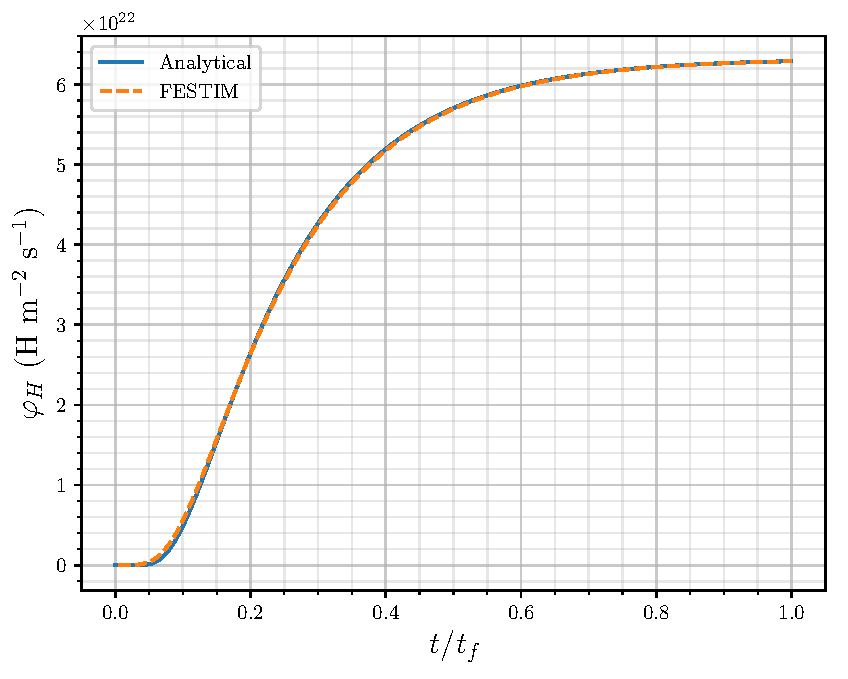
\includegraphics[width=\linewidth]{Figures/Chapter3/FESTIM_vs_analytical.pdf}
    \caption{Temporal evolution of the particle flux $\varphi_H$ ($t_f = \SI{e-8}{s}$)}
    \label{fig:FESTIM vs analytical}
\end{figure}
\subsubsection{Analytical verification using MMS} \label{mms}

To unravel the complexity of governing equations, the Method of Manufactured Solutions (MMS) is often used \sidecite{dudson_verification_2016, roache_code_2002}.
Manufactured solutions are exact solutions that have been modified with additional source terms.
The sets of source terms and boundary conditions obtained are then fed into FESTIM and the error is measured.


At this extent the following manufactured solutions are chosen:
\begin{equation}
    \begin{cases}
    c_{m_D} = 1 + x^2 + \sin(t) \\
    c_{{t,1}_D} = 1 + x^2 + \cos(t)
    \end{cases}
    \label{eq: manufactured solutions}
\end{equation}

By combining Equations \ref{eq:mobile}, \ref{eq:trapped} and \ref{eq: manufactured solutions}, one can obtain the following source terms:
\begin{equation}
    \begin{cases}
    f = \cos(t) - \sin(t) - 2D \\
    g_1 = \nu_1 c_{{t,1}_D} - \nu_m c_{m_D} ( n_1 - c_{{t,1}_D}) - \sin(t)
    \end{cases}
    \label{eq:sources}
\end{equation}

where $g_1$ is an additional source term in Equation \ref{eq:trapped}.
The Dirichlet boundary conditions for $c_m$ and $c_{t,1}$ are:

\begin{equation}
    \begin{cases}
    c_m = 1 + x^2 + \sin(t) \quad \text{on } \partial \Omega \\
    c_{t,1} = 1 + x^2 + \cos(t) \quad \text{on } \partial \Omega 
    \end{cases}
\end{equation}
where $\partial\Omega$ is the boundary of the domain.
Finally, initial values for $c_m$ and $c_{t,i}$ are:
\begin{equation}
    \begin{cases}
    c_m(t=0) = 1 + x^2 \\
    c_{t,1}(t=0) = 2 + x^2
    \end{cases}
\end{equation}
Once all these parameters are fed into FESTIM, one can easily compare the computed solution with the exact solution in Equation \ref{eq: manufactured solutions}.
The L2-norm $E_{c_m}$ can then be calculated as follow:
\begin{equation}
    E_{c_m} = \sqrt{\int_\Omega(c_{m_D} - c_m)^2dx}
\end{equation}
The evolution of $E_{c_m}$ as function of the element size $h$ is shown on Figure \ref{fig:error vs h}.
One can notice that $E_{c_m}$ increases as $A\cdot h^k$.
This is known as the \textit{asymptotic regime} and the coefficient $k$ is called the convergence rate.
$k$ typically tends to N+1 as $h$ approaches $0$, $N$ being the order of the finite elements.
In this simulation, $k$ approaches $2$ as expected since elements of order $1$ have been used.

\begin{figure}
    \centering
    \includegraphics[width=1\linewidth]{"Figures/Chapter3/L2 error on Cm vs h"}
    \caption{Evolution of the L2 norm of the error as function of element size h}
    \label{fig:error vs h}
\end{figure}

The results of the verification cases studied in Sections \ref{analytical} and \ref{mms} show that FESTIM reliably solves the governing Equations \ref{eq:mobile} and \ref{eq:trapped}.
It has also been shown that the convergence rate is in accordance with the theory of finite elements meaning that the code is free of errors that could lead to unreliable results in the future.
Validation can then be performed to ensure that the MRE model described in Section \ref{description_H_transport_model} can be used to reproduce experimental results.